Currently if someone is trying to adjust their shutters they have to manually adjust their shutters by moving them up or down. We aim to create a product that automates this process. The user would be able to adjust how much light gets in through the shutters on an app, this app would connect over a proprietary connection to a hub. The hub will be connected to multiple individual shutters allowing a user to adjust multiple shutters at once or individually adjust each shutter. The app would be able to send a signal to the shutter which would allow the shutter tilts to increase or reduce the light that is let into the room.
\begin{figure}[t]
    \centering
    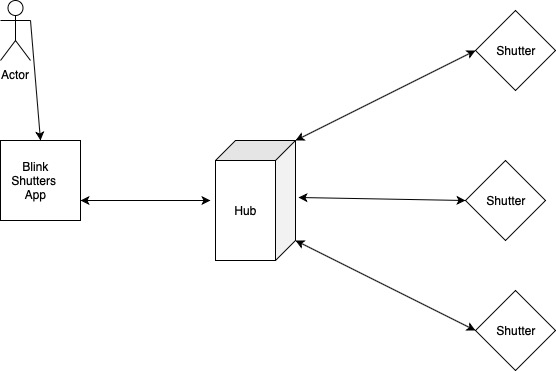
\includegraphics[width=0.5\textwidth]{images/SystemOverview}
    \caption{System Overview}
\end{figure}